%! TEX program = xelatex
%! TEX root = ../root.tex

\section{实验原理}
\subsection{CSR指令}
实现RSIC-V的中断与异常首先就需要能够对CSR进行读写操作,M特权模式提供了如下六种指令进行操作。\\

\begin{figure}[H] %H为当前位置,!htb为忽略美学标准,htbp为浮动图形
    \centering %图片居中
    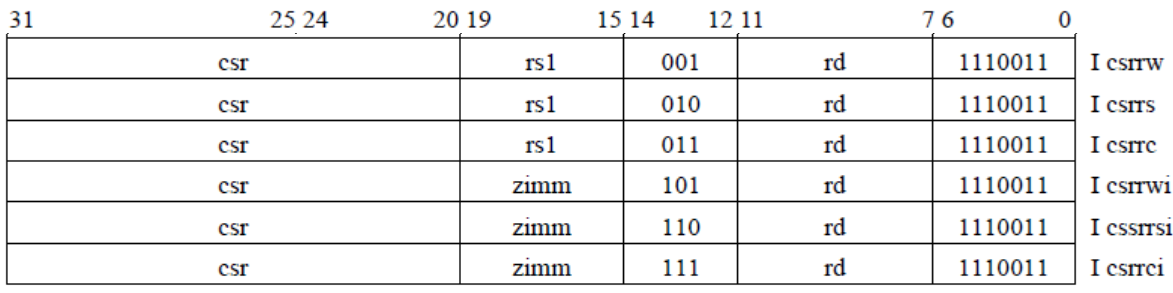
\includegraphics[width=1.0\textwidth]{figs/csr.png} %插入图片,[]中设置图片大小,{}中是图片文件名
    \caption{CSR指令} %最终文档中希望显示的图片标题
    \label{Fig.1} %用于文内引用的标签
\end{figure}

介绍完指令格式之后,CSR每个指令的作用如下\\

\begin{tabular}{|l|l|l|}
    \hline
    操作名 & 使用方式 & 操作方式\\
    \hline
    csrrw & csrrw rd, csr, rs1 & t = CSRs[csr]; CSRs[csr] = x[rs1]; x[rd] = t \\
    \hline
    csrrs & csrrs rd, csr, rs1 & t = CSRs[csr]; CSRs[csr] = t | x[rs1]; x[rd] = t \\
    \hline
    csrrc & csrrc rd, csr, rs1  & t = CSRs[csr]; CSRs[csr] = t \& ~x[rs1]; x[rd] = t \\
    \hline
    csrrwi & csrrwi rd, csr, zimm[4:0] & x[rd] = CSRs[csr]; CSRs[csr] = zimm \\
    \hline
    csrrsi & csrrsi rd, csr, zimm[4:0] & t = CSRs[csr]; CSRs[csr] = t | zimm; x[rd] = t \\
    \hline 
    csrrci & csrrci rd, csr, zimm[4:0] & t = CSRs[csr]; CSRs[csr] = t \& ~zimm; x[rd] = t \\
    \hline
\end{tabular} \\

\subsection{CSR寄存器}
RISC-V定义了一些控制和状态寄存器(CSR),用于配置或记录一些运行的状态,而CSR寄存器是处理器内核内部的寄存器,使用专有的12位地址编码空间,此次实验使用到了下述寄存器

\begin{figure}[H] %H为当前位置,!htb为忽略美学标准,htbp为浮动图形
    \centering %图片居中
    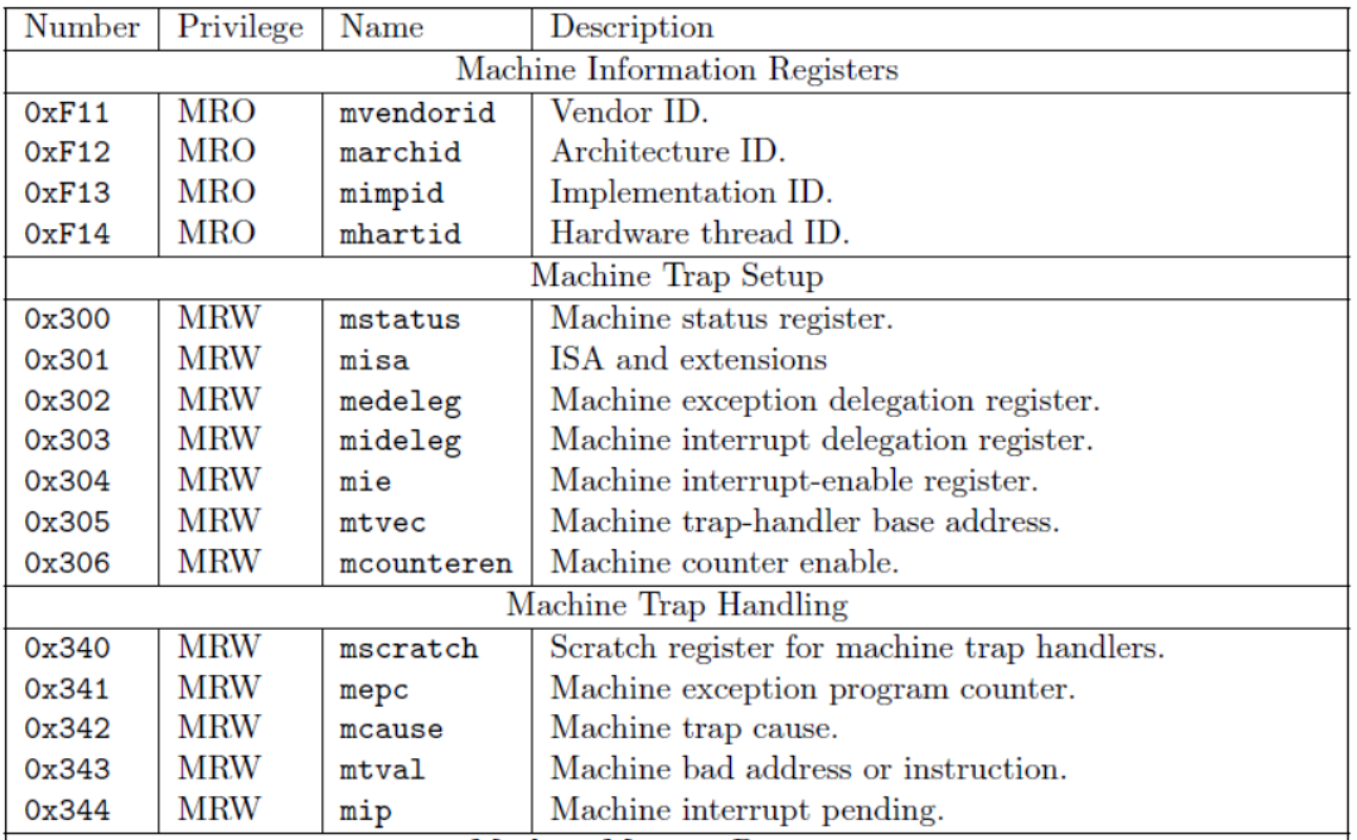
\includegraphics[width=1.0\textwidth]{figs/csrregs.png} %插入图片,[]中设置图片大小,{}中是图片文件名
    \caption{CSR寄存器} %最终文档中希望显示的图片标题
    \label{Fig.2} %用于文内引用的标签
\end{figure}

下面对各个控制与状态寄存器做具体的描述:
\subparagraph{mtvec}
Riscv处理器trap后跳入的PC地址由一个叫做机器模式异常入口基地址寄存器mtvec的csr寄存器指定。mtvec是一个可读可写的寄存器,软件可以编程设定它的值。

\begin{figure}[H] %H为当前位置,!htb为忽略美学标准,htbp为浮动图形
    \centering %图片居中
    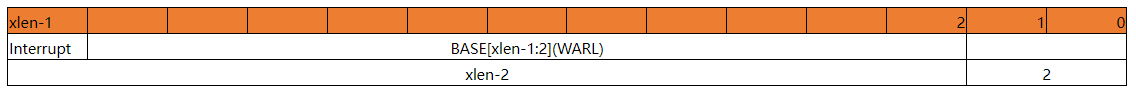
\includegraphics[width=1.0\textwidth]{figs/mtvec.png} %插入图片,[]中设置图片大小,{}中是图片文件名
    \caption{mtvec} %最终文档中希望显示的图片标题
    \label{Fig.3} %用于文内引用的标签
\end{figure}

\begin{itemize}
    \item [1.] 假设mode的值为0,则所有的异常响应时处理器均跳转到base值指示的pc地址
    \item [2.] 假设mode的值为1,则狭义的异常发生时候,处理器均跳转到base值指示的pc地址。狭义的中断发生时候,处理器跳转到base+4*cause值指示的pc地址。cause的值表示中断对应的异常编号(exception code)。
\end{itemize}

\subparagraph{mcause}
Riscv架构规定,进入异常时候,机器模式异常原因寄存器mcause被同时更新,以反映当前的异常种类,软件可以通过读此寄存器查询造成异常的具体原因。

\begin{figure}[H] %H为当前位置,!htb为忽略美学标准,htbp为浮动图形
    \centering %图片居中
    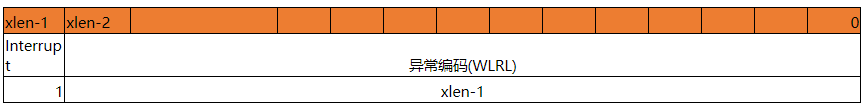
\includegraphics[width=1.0\textwidth]{figs/mcause.png} %插入图片,[]中设置图片大小,{}中是图片文件名
    \caption{mcause} %最终文档中希望显示的图片标题
    \label{Fig.4} %用于文内引用的标签
\end{figure}

异常编号域定义了中断和异常类型,如下表所示:

\begin{figure}[H] %H为当前位置,!htb为忽略美学标准,htbp为浮动图形
    \centering %图片居中
    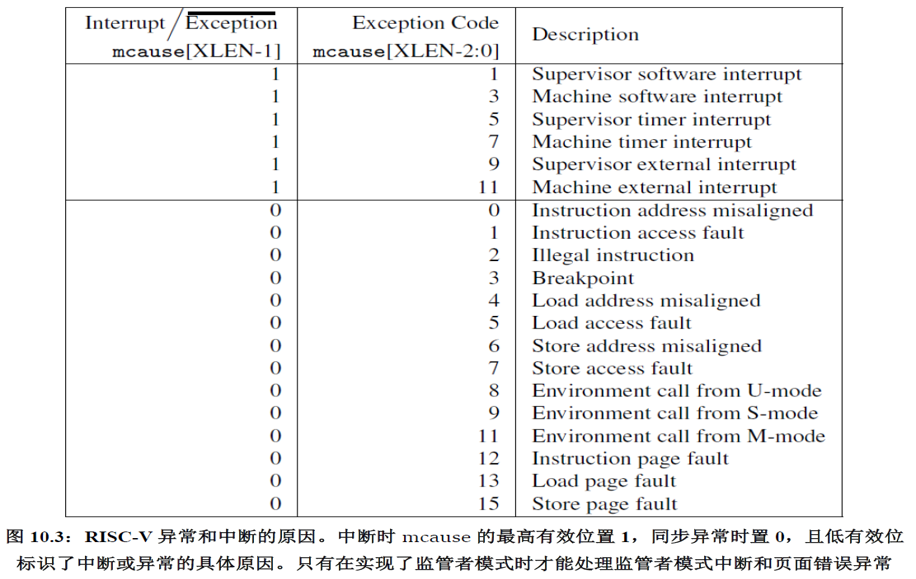
\includegraphics[width=1.0\textwidth]{figs/cause.png} %插入图片,[]中设置图片大小,{}中是图片文件名
    \caption{cause} %最终文档中希望显示的图片标题
    \label{Fig.5} %用于文内引用的标签
\end{figure}

\subparagraph{mepc}
Riscv架构定义异常的返回地址由机器模式异常PC寄存器mepc保存。在进入异常时候,硬件将自动更新mepc寄存器的值为当前遇到异常的指令PC值(即当前程序的停止执行点)。该寄存器的值将作为异常的返回地址,在异常结束后,能够使用它保存的pc值返回之前停止执行的程序点。注意:mepc虽然被自动更新,但它是可读可写的,软件可以直接读写该寄存器的值。

\begin{figure}[H] %H为当前位置,!htb为忽略美学标准,htbp为浮动图形
    \centering %图片居中
    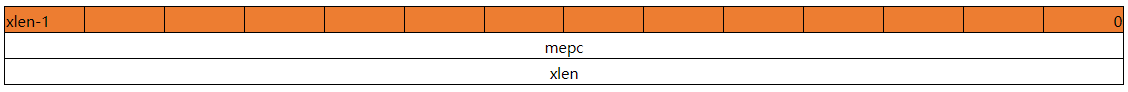
\includegraphics[width=1.0\textwidth]{figs/mepc.png} %插入图片,[]中设置图片大小,{}中是图片文件名
    \caption{mepc} %最终文档中希望显示的图片标题
    \label{Fig.6} %用于文内引用的标签
\end{figure}

出现中断时候,中断返回地址mepc的值被更新为下一条尚未执行的指令。出现异常时候,中断返回地址mepc的值被更新为当前发生异常的指令pc。注意:如果异常是有ecall和ebreak产生,由于mepc的值被更新为ecall或者ebreak指令自己的PC。因此,在异常返回时候,如果直接使用mepc保存的pc值作为返回地址,则会再次进入异常,形成死循环。正确的做法是在异常处理程序中软件改变mepc指向下一条指令。

\subparagraph{mtval}
Riscv规定,在进入异常时候,硬件将自动更新机器模式异常值寄存器mtval,以反映引起当前异常的存储器访问地址或者指令编码。

\begin{figure}[H] %H为当前位置,!htb为忽略美学标准,htbp为浮动图形
    \centering %图片居中
    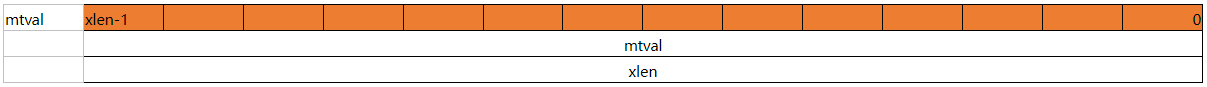
\includegraphics[width=1.0\textwidth]{figs/mtval.png} %插入图片,[]中设置图片大小,{}中是图片文件名
    \caption{mtval} %最终文档中希望显示的图片标题
    \label{Fig.7} %用于文内引用的标签
\end{figure}

如果是由访问存储器造成的异常,比如硬件断点,取指令,存储器读写造成的异常,则将存储器访问的地址更新到mtval。如果是由非法指令造成的异常,则将该指令的指令编码更新到mtval寄存器中。

\subparagraph{mstatus}
mstatus是机器模式下的状态寄存器。

\begin{figure}[H] %H为当前位置,!htb为忽略美学标准,htbp为浮动图形
    \centering %图片居中
    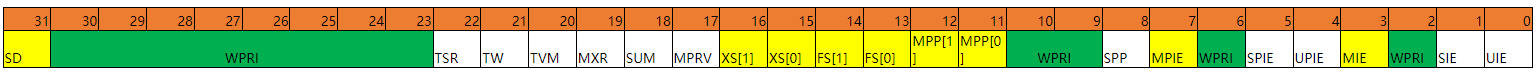
\includegraphics[width=1.0\textwidth]{figs/mstatus.png} %插入图片,[]中设置图片大小,{}中是图片文件名
    \caption{mstatus} %最终文档中希望显示的图片标题
    \label{Fig.8} %用于文内引用的标签
\end{figure}

MIE域表示全局中断使能。当该MIE域值为1时,表示所有中断的全局开关打开,当MIE域的值为0时候,表示全局关闭所有中断。
MPIE用于保存进入异常之前MIE域的值。
MPP用于保存进入异常之前特权模式的值。
处理器进入异常时候:MPIE域的值被更新为MIE的值。MIE的值被更新为0(意味着进入异常,中断被屏蔽)。
MPP的值被更新为异常发生前的模式(如果只实现机器模式,则MPP的值永远为11)。

\subparagraph{mie/mip}
Riscv架构上定义的异常是不可屏蔽的,但狭义上的中断是可以屏蔽的,通过设置mie寄存器来屏蔽中断。mip寄存器用于查询中断的等待状态,软件可以通过读mip寄存器达到查询中断状态的结果。

\begin{figure}[H] %H为当前位置,!htb为忽略美学标准,htbp为浮动图形
    \centering %图片居中
    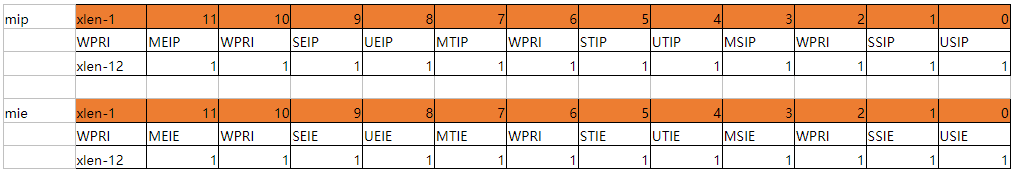
\includegraphics[width=1.0\textwidth]{figs/mipmie.png} %插入图片,[]中设置图片大小,{}中是图片文件名
    \caption{mipmie} %最终文档中希望显示的图片标题
    \label{Fig.9} %用于文内引用的标签
\end{figure}

机器模式下外部中断的屏蔽由csr寄存器mie中MEIE域控制,等待标志(pending)则反映在csr寄存器mip的MEIP域。mip和mie寄存器的高20位可以用于扩展其它的自定义中断类型。

\subsection{处理过程}
发生异常/中断时,硬件自动经历如下的状态转换:
\begin{itemize}
    \item [1.] 异常指令的PC被保存在mepc中,PC被设置为mtvec。mepc指向导致异常的指令;对于中断,它指向中断处理后应该恢复执行的位置。
    \item [2.] 根据异常来源设置mcause,并将mtval设置为出错的地址或者其它适用于特定异常的信息字。
    \item [3.] 把控制状态寄存器mstatus中的MIE位置零以禁用中断,并把先前的MIE值保留到MPIE中。
    \item [4.] 发生异常之前的权限模式保留在mstatus的MPP域中,再把权限模式更改为M。
\end{itemize}

从中断与异常处理返回时需要用到mret指令,处理过程如下:
\begin{itemize}
    \item [1.] PC被设置为mepc
    \item [2.] 恢复mstatus的MIE位
    \item [3.] 恢复保存在mstatus的MPP域中的权限模式
\end{itemize}

\subsection{精确Exception}
在本次实验中,我们实现的是精确异常。也即异常所有之前的指令必须回收,异常之后的指令之后的指令一律不得回收,即不可以更新体系结构状态。
为实现这一要求,我们做了如下设计:
\begin{itemize}
    \item [1.] 所以异常的跳转均需要在WB阶段进行,也就是说前几个阶段侦测到的异常不会立刻进入异常处理,而是要流入WB后再同一处理
    \item [2.] 如果多阶段产生了异常,处理最早产生的异常
    \item [3.] 使用异常向量来完成这一操作:如果异常被检测到异常信号将会被加入异常向量并且取消所有修改系统状态的写信号
\end{itemize}

根据上述原理,我组设计的中断异常模块如下:
\begin{lstlisting}[language = {verilog}]
`timescale 1ns / 1ps

module ExceptionUnit(
	input clk, rst,
	input csr_rw_in,
	input[1:0] csr_wsc_mode_in,
	input csr_w_imm_mux,
	input[11:0] csr_rw_addr_in,
	input[31:0] csr_w_data_reg,
	input[4:0] csr_w_data_imm,
	output[31:0] csr_r_data_out,
	
	input interrupt,
	input illegal_inst,
	input l_access_fault,
	input s_access_fault,
	input ecall_m,
	input[31:0] faultaddr,
	input[31:0] faultInst,
	input mret,
	
	input[31:0] epc_cur,
	input inst_is_zero,
	input[31:0] epc_next,
	output [31:0] PC_redirect,
	output redirect_mux,
	
	output reg_FD_flush, reg_DE_flush, reg_EM_flush, reg_MW_flush, 
	output RegWrite_cancel
);

	wire [31:0] wdata;
	
	reg[31:0] CSR [0:15];
	
	wire ex_in=interrupt|illegal_inst|l_access_fault|s_access_fault|ecall_m;
	localparam mstatus = 0;
	localparam mie     = 4;
	localparam mtvec   = 5;
	localparam mepc    = 9;
	localparam mcause  = 10;
	localparam mtval   = 11;
	localparam mip     = 12;
	
	// Address mapping. The address is 12 bits, but only 4 bits are used in this module.
	wire raddr_valid = csr_rw_addr_in[11:7] == 5'h6 && csr_rw_addr_in[5:3] == 3'h0;
	wire[3:0] raddr_map = (csr_rw_addr_in[6] << 3) + csr_rw_addr_in[2:0];
	wire waddr_valid = csr_rw_addr_in[11:7] == 5'h6 && csr_rw_addr_in[5:3] == 3'h0;
	wire[3:0] waddr_map = (csr_rw_addr_in[6] << 3) + csr_rw_addr_in[2:0];
	
	assign csr_r_data_out = CSR[raddr_map];
	assign wdata = csr_w_imm_mux ? csr_w_data_imm : csr_w_data_reg;
	
	//According to the diagram, design the Exception Unit
	always@(posedge clk or posedge rst)begin
		if(rst) begin
			CSR[0] = 32'h88;
			CSR[1] = 0;
			CSR[2] = 0;
			CSR[3] = 0;
			CSR[4] = 32'hfff;
			CSR[5] = 0;
			CSR[6] = 0;
			CSR[7] = 0;
			CSR[8] = 0;
			CSR[9] = 0;
			CSR[10] = 0;
			CSR[11] = 0;
			CSR[12] = 0;
			CSR[13] = 0;
			CSR[14] = 0;
			CSR[15] = 0;
		end
		else if(csr_rw_in && ~ex_in) begin
			case(csr_wsc_mode_in)
				2'b01: CSR[waddr_map] = wdata;
				2'b10: CSR[waddr_map] = CSR[waddr_map] | wdata;
				2'b11: CSR[waddr_map] = CSR[waddr_map] & ~wdata;
				default: CSR[waddr_map] = wdata;
			endcase            
		end
		else if(ex_in && CSR[mstatus][3]==1 && ~inst_is_zero ) begin
			CSR[mepc] = interrupt ? epc_next : epc_cur ;
			if (interrupt) begin
				CSR[mcause]=32'h800b;
			end 
			else begin
				if(ecall_m) CSR[mcause]=32'hb;
				else if(s_access_fault) CSR[mcause]=32'h6;
				else if(l_access_fault) CSR[mcause]=32'h4;
				else if(illegal_inst) CSR[mcause]=32'h2;
			end
			if (~interrupt) begin
				if(ecall_m) CSR[mtval]=0;
				else if(s_access_fault) CSR[mtval]=faultaddr;
				else if(l_access_fault) CSR[mtval]=faultaddr;
				else if(illegal_inst) CSR[mtval]=faultInst;
			end
			CSR[mstatus][7]=CSR[mstatus][3];
			CSR[mstatus][3]=0;
		end  
		else if(mret) begin;
			CSR[mstatus][3]=CSR[mstatus][7];
		end     
	end
	
	assign PC_redirect = (ex_in & CSR[mstatus][3] & ~inst_is_zero) ? CSR[mtvec] :
						mret ? CSR[mepc] : 0;
	assign redirect_mux = (ex_in & CSR[mstatus][3] & ~inst_is_zero) | mret;
	assign reg_FD_flush= (ex_in & CSR[mstatus][3] & ~inst_is_zero)|mret;
	assign reg_DE_flush= (ex_in & CSR[mstatus][3] & ~inst_is_zero)|mret;
	assign reg_EM_flush= (ex_in & CSR[mstatus][3] & ~inst_is_zero)|mret; 
	assign reg_MW_flush= (ex_in & CSR[mstatus][3] & ~inst_is_zero)|mret; 
	assign RegWrite_cancel= ex_in & CSR[mstatus][3] & ~inst_is_zero;

endmodule
\end{lstlisting}

\subsection{数据通路}
完成了个部件的设计,数据通路就是将各个部分连接起来,保证各功能正常实现的关键部分,下面是总体的原理图

\begin{figure}[H] %H为当前位置,!htb为忽略美学标准,htbp为浮动图形
    \centering %图片居中
    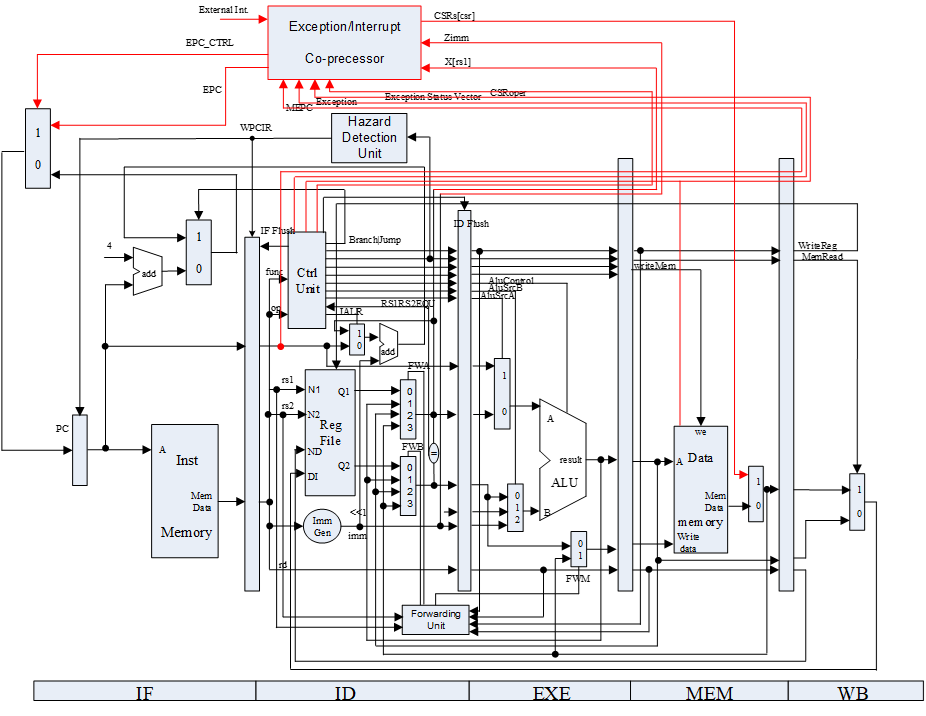
\includegraphics[width=1.0\textwidth]{figs/DataPath.png} %插入图片,[]中设置图片大小,{}中是图片文件名
    \caption{DataPath} %最终文档中希望显示的图片标题
    \label{Fig.10} %用于文内引用的标签
\end{figure}

数据通路的补充就是根据原理图连线即可,具体的源代码如下
\begin{lstlisting}[language = {verilog}]
`timescale 1ns / 1ps


module  RV32core(
        input debug_en,  // debug enable
        input debug_step,  // debug step clock
        input [6:0] debug_addr,  // debug address
        output[31:0] debug_data,  // debug data
        input clk,  // main clock
        input rst,  // synchronous reset
        input interrupter  // interrupt source, for future use
    );

    wire debug_clk;

    debug_clk clock(.clk(clk),.debug_en(debug_en),.debug_step(debug_step),.debug_clk(debug_clk));

    wire Branch_ctrl, JALR, RegWrite_ctrl, mem_w_ctrl, mem_r_ctrl,
        ALUSrc_A_ctrl, ALUSrc_B_ctrl, DatatoReg_ctrl, rs1use_ctrl, rs2use_ctrl,
        MRET, csr_rw_ctrl, csr_w_imm_mux_ctrl;
    wire[1:0] hazard_optype_ctrl, exp_vector_ctrl;
    wire[2:0] ImmSel_ctrl, cmp_ctrl;
    wire[3:0] ALUControl_ctrl;

    wire forward_ctrl_ls;
    wire[1:0] forward_ctrl_A, forward_ctrl_B;

    wire PC_EN_IF;
    wire [31:0] PC_IF, next_PC_IF, PC_4_IF, inst_IF, final_PC_IF;

    wire reg_FD_stall, reg_FD_flush, isFlushed_ID, cmp_res_ID;
    wire [31:0] jump_PC_ID, PC_ID, inst_ID, Debug_regs, rs1_data_reg, rs2_data_reg,
        Imm_out_ID, rs1_data_ID, rs2_data_ID, addA_ID;
    
    wire reg_DE_flush, isFlushed_EXE, RegWrite_EXE, mem_w_EXE, mem_r_EXE,
        ALUSrc_A_EXE, ALUSrc_B_EXE, ALUzero_EXE, ALUoverflow_EXE, DatatoReg_EXE,
        csr_rw_EXE, csr_w_imm_mux_EXE, mret_EXE;
    wire[1:0] exp_vector_EXE;
    wire[2:0] u_b_h_w_EXE;
    wire[3:0] ALUControl_EXE;
    wire[4:0] rs1_EXE, rs2_EXE, rd_EXE;
    wire[31:0] ALUout_EXE, PC_EXE, inst_EXE, rs1_data_EXE, rs2_data_EXE, Imm_EXE,
        ALUA_EXE, ALUB_EXE, Dataout_EXE;

    wire redirect_mux_exp, reg_FD_flush_exp, reg_DE_flush_exp,
        reg_EM_flush_exp, reg_MW_flush_exp, RegWrite_cancel_exp;
    wire[31:0] PC_redirect_exp;
    
    wire isFlushed_MEM, RegWrite_MEM, DatatoReg_MEM, mem_w_MEM, mem_r_MEM,
        csr_rw_MEM, csr_w_imm_mux_MEM, mret_MEM, l_access_fault_MEM, s_access_fault_MEM;
    wire[1:0] exp_vector_MEM;
    wire[2:0] u_b_h_w_MEM;
    wire[4:0] rs1_MEM, rd_MEM;
    wire[31:0] ALUout_MEM, PC_MEM, inst_MEM, Dataout_MEM, Datain_MEM,
        rs1_data_MEM, CSRout_MEM, RAMout_MEM;


    wire isFlushed_WB, RegWrite_WB, DatatoReg_WB;
    wire[3:0] exp_vector_WB;
    wire[4:0] rd_WB;
    wire [31:0] wt_data_WB, PC_WB, inst_WB, ALUout_WB, Datain_WB;


    // IF
    REG32 REG_PC(.clk(debug_clk),.rst(rst),.CE(PC_EN_IF),.D(final_PC_IF),.Q(PC_IF));
    
    add_32 add_IF(.a(PC_IF),.b(32'd4),.c(PC_4_IF));

    MUX2T1_32 mux_IF(.I0(PC_4_IF),.I1(jump_PC_ID),.s(Branch_ctrl),.o(next_PC_IF));

    MUX2T1_32 redirectPC(.I0(next_PC_IF),.I1(PC_redirect_exp),.s(redirect_mux_exp),.o(final_PC_IF));

    ROM_D inst_rom(.a(PC_IF[8:2]),.spo(inst_IF));


    // ID
    REG_IF_ID reg_IF_ID(.clk(debug_clk),.rst(rst),.EN(1'b1),.Data_stall(reg_FD_stall),
        .flush(reg_FD_flush | reg_FD_flush_exp),.PCOUT(PC_IF),.IR(inst_IF),

        .IR_ID(inst_ID),.PCurrent_ID(PC_ID),.isFlushed(isFlushed_ID));
    
    CtrlUnit ctrl(.inst(inst_ID),.cmp_res(cmp_res_ID),.Branch(Branch_ctrl),.ALUSrc_A(ALUSrc_A_ctrl),
        .ALUSrc_B(ALUSrc_B_ctrl),.DatatoReg(DatatoReg_ctrl),.RegWrite(RegWrite_ctrl),
        .mem_w(mem_w_ctrl),.mem_r(mem_r_ctrl),.rs1use(rs1use_ctrl),.rs2use(rs2use_ctrl),
        .hazard_optype(hazard_optype_ctrl),.ImmSel(ImmSel_ctrl),.cmp_ctrl(cmp_ctrl),
        .ALUControl(ALUControl_ctrl),.JALR(JALR),.MRET(MRET),.csr_rw(csr_rw_ctrl),
        .csr_w_imm_mux(csr_w_imm_mux_ctrl),.exp_vector(exp_vector_ctrl));
    
    Regs register(.clk(debug_clk),.rst(rst),.L_S(RegWrite_WB & ~RegWrite_cancel_exp),
        .R_addr_A(inst_ID[19:15]),.R_addr_B(inst_ID[24:20]),
        .rdata_A(rs1_data_reg),.rdata_B(rs2_data_reg),
        .Wt_addr(rd_WB),.Wt_data(wt_data_WB),
        .Debug_addr(debug_addr[4:0]),.Debug_regs(Debug_regs));
    
    ImmGen imm_gen(.ImmSel(ImmSel_ctrl),.inst_field(inst_ID),.Imm_out(Imm_out_ID));
    
    MUX4T1_32 mux_forward_A(.I0(rs1_data_reg),.I1(ALUout_EXE),.I2(ALUout_MEM),.I3(Datain_MEM),
        .s(forward_ctrl_A),.o(rs1_data_ID));
    
    MUX4T1_32 mux_forward_B(.I0(rs2_data_reg),.I1(ALUout_EXE),.I2(ALUout_MEM),.I3(Datain_MEM),
        .s(forward_ctrl_B),.o(rs2_data_ID));
    
    MUX2T1_32 mux_branch_ID(.I0(PC_ID),.I1(rs1_data_ID),.s(JALR),.o(addA_ID));

    add_32 add_branch_ID(.a(addA_ID),.b(Imm_out_ID),.c(jump_PC_ID));

    cmp_32 cmp_ID(.a(rs1_data_ID),.b(rs2_data_ID),.ctrl(cmp_ctrl),.c(cmp_res_ID));
    
    HazardDetectionUnit hazard_unit(.clk(debug_clk),.Branch_ID(Branch_ctrl),.rs1use_ID(rs1use_ctrl),
        .rs2use_ID(rs2use_ctrl),.hazard_optype_ID(hazard_optype_ctrl),.rd_EXE(rd_EXE),
        .rd_MEM(rd_MEM),.rs1_ID(inst_ID[19:15]),.rs2_ID(inst_ID[24:20]),.rs2_EXE(rs2_EXE),
        .PC_EN_IF(PC_EN_IF),.reg_FD_stall(reg_FD_stall),.reg_FD_flush(reg_FD_flush),
        .reg_DE_flush(reg_DE_flush),.forward_ctrl_ls(forward_ctrl_ls),.forward_ctrl_A(forward_ctrl_A),
        .forward_ctrl_B(forward_ctrl_B));


    // EX
    REG_ID_EX reg_ID_EX(.clk(debug_clk),.rst(rst),.EN(1'b1),
        .flush(reg_DE_flush | reg_DE_flush_exp | isFlushed_ID),
        .IR_ID(inst_ID),.PCurrent_ID(PC_ID),.rs1_addr(inst_ID[19:15]),.rs2_addr(inst_ID[24:20]),
        .rs1_data(rs1_data_ID),.rs2_data(rs2_data_ID),.Imm32(Imm_out_ID),.rd_addr(inst_ID[11:7]),
        .ALUSrc_A(ALUSrc_A_ctrl),.ALUSrc_B(ALUSrc_B_ctrl),.ALUC(ALUControl_ctrl),.DatatoReg(DatatoReg_ctrl),
        .RegWrite(RegWrite_ctrl),.WR(mem_w_ctrl),.u_b_h_w(inst_ID[14:12]),.mem_r(mem_r_ctrl),
        .csr_rw(csr_rw_ctrl),.csr_w_imm_mux(csr_w_imm_mux_ctrl),.mret(MRET),
        .exp_vector(exp_vector_ctrl),

        .PCurrent_EX(PC_EXE),.IR_EX(inst_EXE),.rs1_EX(rs1_EXE),.rs2_EX(rs2_EXE),
        .A_EX(rs1_data_EXE),.B_EX(rs2_data_EXE),.Imm32_EX(Imm_EXE),.rd_EX(rd_EXE),
        .ALUSrc_A_EX(ALUSrc_A_EXE),.ALUSrc_B_EX(ALUSrc_B_EXE),.ALUC_EX(ALUControl_EXE),
        .DatatoReg_EX(DatatoReg_EXE),.RegWrite_EX(RegWrite_EXE),.WR_EX(mem_w_EXE),
        .u_b_h_w_EX(u_b_h_w_EXE),.mem_r_EX(mem_r_EXE),.isFlushed(isFlushed_EXE),
        .csr_rw_EX(csr_rw_EXE),.csr_w_imm_mux_EX(csr_w_imm_mux_EXE),.mret_EX(mret_EXE),
        .exp_vector_EX(exp_vector_EXE));
    
    MUX2T1_32 mux_A_EXE(.I0(rs1_data_EXE),.I1(PC_EXE),.s(ALUSrc_A_EXE),.o(ALUA_EXE));

    MUX2T1_32 mux_B_EXE(.I0(rs2_data_EXE),.I1(Imm_EXE),.s(ALUSrc_B_EXE),.o(ALUB_EXE));

    ALU alu(.A(ALUA_EXE),.B(ALUB_EXE),.Control(ALUControl_EXE),
        .res(ALUout_EXE),.zero(ALUzero_EXE),.overflow(ALUoverflow_EXE));
    
    MUX2T1_32 mux_forward_EXE(.I0(rs2_data_EXE),.I1(Datain_MEM),.s(forward_ctrl_ls),.o(Dataout_EXE));


    // MEM
    REG_EX_MEM reg_EXE_MEM(.clk(debug_clk),.rst(rst),.EN(1'b1),.flush(reg_EM_flush_exp | isFlushed_EXE),
        .IR_EX(inst_EXE),.PCurrent_EX(PC_EXE),.ALUO_EX(ALUout_EXE),.B_EX(Dataout_EXE),
        .rd_EX(rd_EXE),.rs1_EX(rs1_EXE),.rs1_data_EX(rs1_data_EXE),.DatatoReg_EX(DatatoReg_EXE),
        .RegWrite_EX(RegWrite_EXE),.WR_EX(mem_w_EXE),.u_b_h_w_EX(u_b_h_w_EXE),.mem_r_EX(mem_r_EXE),
        .csr_rw_EX(csr_rw_EXE),.csr_w_imm_mux_EX(csr_w_imm_mux_EXE),.mret_EX(mret_EXE),
        .exp_vector_EX(exp_vector_EXE),

        .PCurrent_MEM(PC_MEM),.IR_MEM(inst_MEM),.ALUO_MEM(ALUout_MEM),.Datao_MEM(Dataout_MEM),
        .rd_MEM(rd_MEM),.rs1_MEM(rs1_MEM),.rs1_data_MEM(rs1_data_MEM),.DatatoReg_MEM(DatatoReg_MEM),
        .RegWrite_MEM(RegWrite_MEM),.WR_MEM(mem_w_MEM),.u_b_h_w_MEM(u_b_h_w_MEM),.mem_r_MEM(mem_r_MEM),
        .isFlushed(isFlushed_MEM),.csr_rw_MEM(csr_rw_MEM),.csr_w_imm_mux_MEM(csr_w_imm_mux_MEM),
        .mret_MEM(mret_MEM),.exp_vector_MEM(exp_vector_MEM));
    
    RAM_B data_ram(.addra(ALUout_MEM),.clka(debug_clk),.dina(Dataout_MEM), 
        .wea(mem_w_MEM),.rea(mem_r_MEM),.douta(RAMout_MEM),.mem_u_b_h_w(u_b_h_w_MEM),
        .l_access_fault(l_access_fault_MEM),.s_access_fault(s_access_fault_MEM));

    ExceptionUnit exp_unit(.clk(debug_clk),.rst(rst),.csr_rw_in(csr_rw_MEM),.csr_wsc_mode_in(inst_MEM[13:12]),
        .csr_w_imm_mux(csr_w_imm_mux_MEM),.csr_rw_addr_in(inst_MEM[31:20]),
        .csr_w_data_reg(rs1_data_MEM),.csr_w_data_imm(rs1_MEM),
        .csr_r_data_out(CSRout_MEM),

        .interrupt(interrupter),
        .illegal_inst(~isFlushed_WB & exp_vector_WB[3]),
        .ecall_m(~isFlushed_WB & exp_vector_WB[2]),
        .l_access_fault(~isFlushed_WB & exp_vector_WB[1]),
        .s_access_fault(~isFlushed_WB & exp_vector_WB[0]),
        .mret(mret_MEM),
        /*自行添加*/
        .faultaddr(ALUout_WB),
        .inst_is_zero(inst_WB ? 0 : 1),
        .faultInst(inst_WB),
        /*自行添加*/    
        .epc_cur(PC_WB),
        .epc_next(~isFlushed_MEM ? PC_MEM : ~isFlushed_EXE ? PC_EXE :
        ~isFlushed_ID ? PC_ID : PC_IF),
        .PC_redirect(PC_redirect_exp),.redirect_mux(redirect_mux_exp),
        .reg_FD_flush(reg_FD_flush_exp),.reg_DE_flush(reg_DE_flush_exp),
        .reg_EM_flush(reg_EM_flush_exp),.reg_MW_flush(reg_MW_flush_exp),
        .RegWrite_cancel(RegWrite_cancel_exp));
    
    MUX2T1_32 mux_csrout(.I0(RAMout_MEM),.I1(CSRout_MEM),.s(csr_rw_MEM),.o(Datain_MEM));
        

    // WB
    REG_MEM_WB reg_MEM_WB(.clk(debug_clk),.rst(rst),.EN(1'b1),.flush(reg_MW_flush_exp | isFlushed_MEM),
        .IR_MEM(inst_MEM),.PCurrent_MEM(PC_MEM),.ALUO_MEM(ALUout_MEM),.Datai(Datain_MEM),
        .rd_MEM(rd_MEM),.DatatoReg_MEM(DatatoReg_MEM),.RegWrite_MEM(RegWrite_MEM),
        .exp_vector_MEM({exp_vector_MEM, l_access_fault_MEM, s_access_fault_MEM}),

        .PCurrent_WB(PC_WB),.IR_WB(inst_WB),.ALUO_WB(ALUout_WB),.MDR_WB(Datain_WB),
        .rd_WB(rd_WB),.DatatoReg_WB(DatatoReg_WB),.RegWrite_WB(RegWrite_WB),
        .isFlushed(isFlushed_WB),.exp_vector_WB(exp_vector_WB));
    
    MUX2T1_32 mux_WB(.I0(ALUout_WB),.I1(Datain_WB),.s(DatatoReg_WB),.o(wt_data_WB));


    wire [31:0] Test_signal;
    assign debug_data = debug_addr[5] ? Test_signal : Debug_regs;
    
    CPUTEST    U1_3(.PC_IF(PC_IF),
                    .PC_ID(PC_ID),
                    .PC_EXE(PC_EXE),
                    .PC_MEM(PC_MEM),
                    .PC_WB(PC_WB),
                    .PC_next_IF(next_PC_IF),
                    .PCJump(jump_PC_ID),
                    .inst_IF(inst_IF),
                    .inst_ID(inst_ID),
                    .inst_EXE(inst_EXE),
                    .inst_MEM(inst_MEM),
                    .inst_WB(inst_WB),
                    .PCEN(PC_EN_IF),
                    .Branch(Branch_ctrl),
                    .PCSource(Branch_ctrl),
                    .RS1DATA(rs1_data_reg),
                    .RS2DATA(rs2_data_reg),
                    .Imm32(Imm_out_ID),
                    .ImmSel(ImmSel_ctrl),
                    .ALUC(ALUControl_ctrl),
                    .ALUSrc_A(ALUSrc_A_ctrl),
                    .ALUSrc_B(ALUSrc_B_ctrl),
                    .A(ALUA_EXE),
                    .B(ALUB_EXE),
                    .ALU_out(ALUout_MEM),
                    .Datai(Datain_MEM),
                    .Datao(Dataout_MEM),
                    .Addr(Addr),
                    .WR(MWR),
                    .MIO(mem_r_MEM),
                    .WDATA(wt_data_WB),
                    .DatatoReg(DatatoReg_WB),
                    .RegWrite(RegWrite_WB),
                    .data_hazard(reg_FD_stall),
                    .control_hazard(Branch_ctrl),
                    .exp_sig({csr_rw_MEM,2'b0,csr_w_imm_mux_MEM,
                        isFlushed_ID, isFlushed_EXE, isFlushed_MEM, isFlushed_WB,
                        interrupter,3'b0,exp_vector_WB,
                        4'b0,
                        3'b0,redirect_mux_exp,
                        reg_FD_flush_exp,reg_DE_flush_exp,reg_EM_flush_exp,reg_MW_flush_exp,
                        3'b0,RegWrite_cancel_exp}),

                    .Debug_addr(debug_addr[4:0]),
                    .Test_signal(Test_signal)    
                    );

endmodule
\end{lstlisting}